\chapter{Competitive pressure in the Australian economy\label{chap:intro}}

Competitive pressure is key to good economic performance. It pushes prices towards costs. It moves resources to their best uses. It can push firms to come up with good ideas. But in recent years, many people around the world have become concerned that competition is not working as it should.

Is competitive intensity too low in Australia, and is it declining? In which sectors do firms with market power earn high profits, and are those profits to the detriment of consumers? This report evaluates the evidence, and proposes policies that can help increase competitive pressure in Australia.

%\section{The benefits of competition}
%Done well, competition raises productivity and incomes:
%\begin{itemize}
%\item evidence on how competition creates consumer value
%\item evidence on how competition reduces cost
%\item evidence on how competition drives innovation
%\end{itemize}

\section{Long-standing Australian concerns about competition}

Competition is even more important in Australia's remote and relatively small economy than in many other economies. Australia has long paid a `remoteness penalty' of about 10 per cent of GDP\@. Small, remote economies have lower productivity because they cannot exploit economies of scale and specialisation while maintaining strong competitive pressure.%
\footcites{DolmanAusUSProd2007}{BattersbyDistance2006}

%\hl{Quotes to come (Miller, Sims).}

\section{Renewed global concerns about competition}

Around the world, many have expressed concern that competition is no longer working as it should. They worry about consolidation of traditional industries, and the rise of highly profitable tech giants. Market concentration rose in more than two-thirds of US sectors between 1997 and 2012. %
%The largest four firms' market share averaged 32 per cent in 2012, up from 26 per cent in 1997. %
%    \footnote{\textcite[][Figures~2~and~3]{Econtoohigh2016}. More than three-quarters of US sectors have become more concentrated over the last two decades as measured by the Herfindahl index, which is typically calculated as the sum of the squared market shares of all (or the top 50) firms in an industry (\textcite[][pp.~10--15 and Figure~1A]{grullon_larkin_michaely_2015}.}
A third of US corporate revenue is now in industries in which the top four firms' market share is between a third and two-thirds, up from a quarter in 1997.%
   \footnote{\textcite{Econtoohigh2016}. Much of the rise is the result of waves of mergers \parencite[][9]{grullon2016us}.}
%The top four firms' share exceeds 30 per cent in telecommunications, manufacturing, transport and logistics, wholesale trade, retail trade, and finance and insurance. A tenth of revenue is earned in sectors where the largest four firms' market share is over two-thirds, including in telecoms, pharmacies and credit cards.%
%    \footnote{\textcites{Econtoohigh2016}{EquitSteroids2017}[][Figure~4, p.~33]{AutorDorn2017}[][Figure~2]{Econtoohigh2016}.


The rise of the tech giants has also prompted concerns about monopoly power. Much of their success is due to innovative products and services, and they have also intensified the competition facing firms in media, retail and other sectors. But their scale can also become an advantage in its own right: `network effects' can help the firm that hosts the largest number of users, or controls the biggest data sets.%
    \footcites{EzrachiVirtual}{Econsuperstar2016}{FT_Silicon_2016}{FT_GoogleEU_2016}

%Beyond this, there is not much evidence of a global increase in the power of large firms.%
 %   \footnote{\url{https://www.economist.com/news/special-report/21707048-small-group-giant-companiessome-old-some-neware-once-again-dominating-global} \hl{but would be good to have a better reference}. Also note an earlier piece on banking concentration and retail interest rates in the EU that found no increase in rates  \url{https://www.ecb.europa.eu/pub/pdf/scpwps/ecbwp72.pdf?9a66c6493abd792fe1ac0f0b233b1ac3}.}

A range of ills have been linked to the rise of market power. Some are concerned that powerful firms are pushing up prices or squeezing workers,%
\footcite{AutorDorn2017}
contributing to a rise in income inequality,
\footcite{Leigh-triggs-AER}
and holding back investment and innovation.%
\footcites{Econtoohigh2016}{Philippon2017}{CEAcompetitionbriefmay2016}{Economicinnovationgroupdynamism}

%Powerful firms might invest less than firms that face more competition; %
   % \footcite{Philippon2017}.
% they can harm consumers and workers;%
%though increases in market concentration can help consumers if larger firms have lower costs and if competitive pressure remains strong enough that they cut prices.
%Some sectors, like construction, appear to have too many small firms.%
    % \footcites[][Fig~1]{CEAcompetitionbriefmay2016}{AutorDorn2017}
 %   \footnote{\url{https://www.economist.com/news/business/21726714-american-builders-productivity-has-plunged-half-late-1960s-efficiency-eludes?fsrc=scn/tw/te/bl/ed/efficiencyeludestheconstructionindustry}.}
% though much of the decline in competitive pressure appears to predate the slowdown in investment. There is little evidence that waning competition has contributed much to the trend decline in capital intensity and the sharper slowdown in growth in the wake of the financial crisis, the two factors that account for the fall in investment.%
%     \textcite{MinifieChisholmPercival2017}}
% and they can deter innovators and market entrants.%
%     \footnote{\textcite{Economicinnovationgroupdynamism}.}

Not all these concerns have been substantiated. For example, most sectors in the US are not so concentrated as to be of concern to competition regulators,\footcite{antitrustpopulism} and competition is one of many factors affecting consumer prices, wages, inequality, investment, and innovation.
%leading firms in the US spend less time at the top of their markets than they did three decades ago.%
 %   \footcites{NewbasescompadvtBCG}{IllusionsEntrepreneur2010}
But while findings are still emerging, there is good evidence of some increase in market power in the US, and some evidence of its costs. 

Far less has been published about competition in Australia, however. This report assesses evidence on the level, trends and impact of market power on competition in Australia. 

\section{What shapes competition in Australia}

This report analyses competition in the \textbf{non-tradeable}, privately-provided part of the Australian economy. Any analysis of competition in Australia has to start from an understanding of how firms compete.

Perhaps the most important factor is \textbf{economies of scale}: in some sectors, large firms have lower costs than small firms. Those sectors are often served by just a few firms. If scale economies are powerful enough, the market is served by a single firm, a \textbf{natural monopoly}.

\textbf{Heavy regulation} also shapes competition. It can add to the costs of doing business in a sector, particularly for smaller firms. It can also restrain competition between firms (for example, by limiting where rivals can locate or when they open), or limit the number of firms directly.

% Scale economies and regulation, in particular, shape competition:%
% \begin{itemize}
%     \item \textbf{Economies of scale}. Perhaps the most important factor is that in some sectors, large firms have lower costs than small firms do. Those sectors are often served by just a few firms. 
%     \item \textbf{Natural monopoly}. If scale economies are powerful enough, the market is served by a single firm, and that firm is said to be a natural monopoly.
%     \item \textbf{Heavy regulation}. Regulations can add to the costs of doing business in a sector, particularly for smaller firms. They can also restrain competition between firms (for example, by limiting where rivals can locate or when they opening), or they may limit the number of firms directly.
% \end{itemize}

%Competition in a modern economy bears little resemblance to the fiction of countless small firms that make identical goods, take the market price for everything they buy and sell, and earn just enough to stay in business. 
\begin{figure}
   \caption{Much of the economy has low entry barriers, is trade-exposed, or is mostly publicly provided \label{fig:economy_waterfall}}
    \units{Gross value added, \$ billions, 2016-17}
    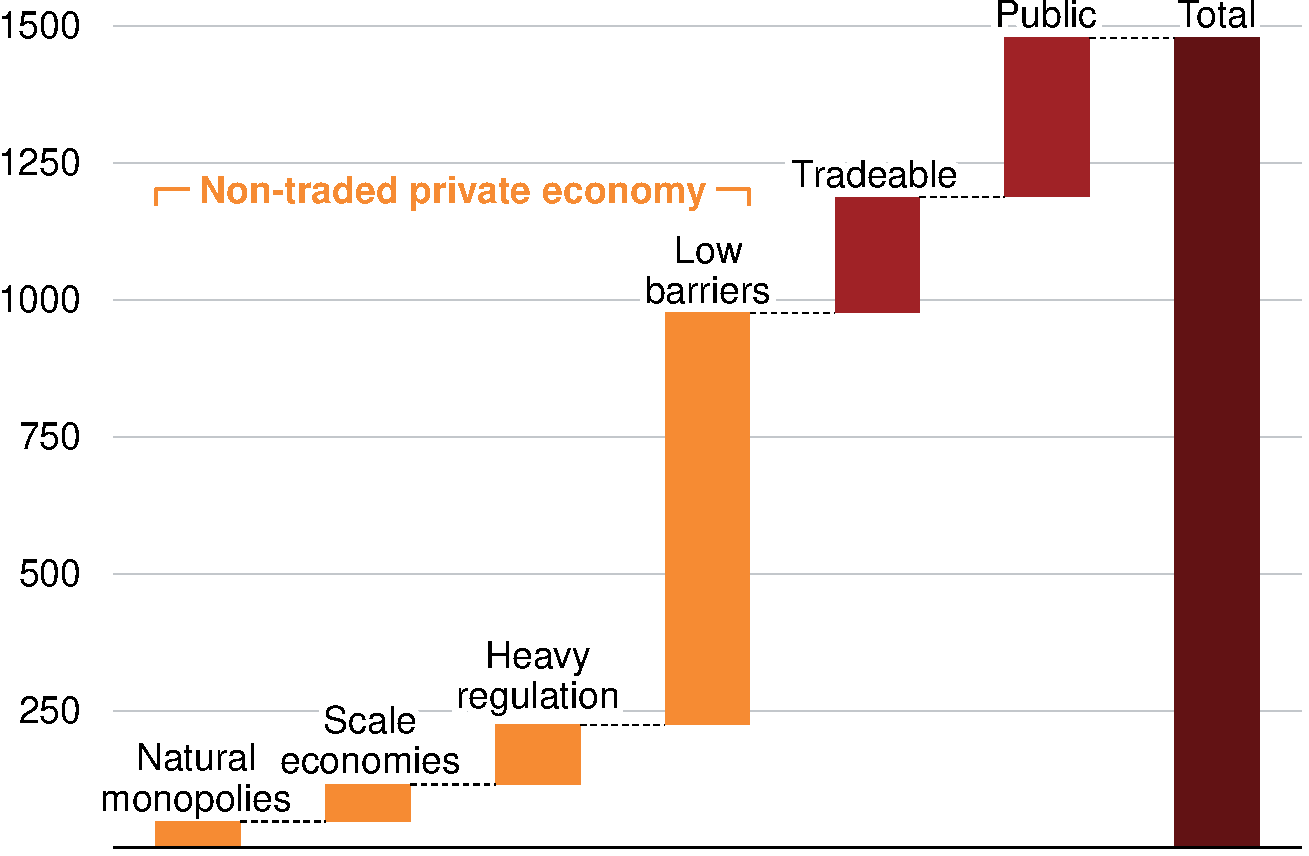
\includegraphics[page=1]{atlas/Charts}
    \noteswithsource{Gross value added is based on the National Accounts published by the ABS\@. Total gross value added differs from gross domestic product because it excludes ownership of dwellings (\$149~billion), and taxes less subsidies on production and imports (\$120~billion). Sector analysis elsewhere in this report uses data published by IBISWorld that omits about 15\% of the non-traded private economy, most of which is in low-barrier sectors. There are also some sector-level discrepancies between IBISWorld and the National Accounts.}{Grattan analysis of \textcites{IBISWorldIndustry2017}{ABS2017SystemNationalAccounts}.}
\end{figure}

This report uses the term \textbf{`barriers to entry'} for these competition-shaping factors. The term is not precise, though it is widely used.%
\footcites{DemsetzBarriersAER1982}{CarltonBarriers2005}{OECDBarriers2007}
In sectors marked by such barriers, there may be fewer actual or potential competitors, or weaker competition.
%But the report does not assume that  barriers weaken competition; instead it looks to the data on profitability as a guide (\Chapref{chap:profits}). 

%Such economies of scale can deter smaller firms from entering the market. Regulation can have a similar effect, protecting incumbent firms in some markets. Behind such barriers, firms can develop and exercise market power.

Sectors marked by such `barriers' are quite a small part of the Australian economy (\Vref{fig:economy_waterfall}). They produce about \$230 billion of gross value added, or about 15 per cent of the total. Of this:%
    \footnote{The allocation of sectors to groups is largely based on industry characterisations made by a commercial provider of industry data \parencite{IBISWorldIndustry2017,IBISWorldCompany2017}, supplemented by our own assessment of industry cost structures and regulation, and so is inherently subjective. Total gross value added (`value added', elsewhere in the report) excludes ownership of dwellings and is for  2016-17.}

\begin{itemize}
    \item The \textbf{natural-monopoly} sectors, where very strong scale economies typically result in a single large firm serving the market, contribute about \$50~billion in value added. These sectors are often regulated, either through direct controls on prices, or through rules obliging their operators to provide access to users.%
        \footnote{Networks for electricity, gas and water supply, for fixed-line telecommunications, rail and road networks, and some ports and airports, are typically natural monopolies.}
    \item The \textbf{scale-economy} sectors, where scale economies are strong enough that a few firms may have large market shares and earn high profits, contribute about \$70~billion in value added. These sectors are typically not highly regulated, but competition law regarding mergers, cartels and misuse of market power often shape how they operate.%
        \footnote{Scale economies may apply over a geographic area, as in retail businesses supported by a logistics hub, or over a network of customers and suppliers, as in internet platforms.}
    \item The \textbf{heavily regulated} sectors, where regulation constrains competition through outright limits, or by imposing costs that disadvantage small firms, contribute about \$110~billion in value added.%
%        \footnote{If regulations impose large enough costs on all firms, they can serve as a `fixed cost' that pushes costs up most for small firms. Fixed tax and compliance costs can be material for small firms. Specific regulations apply to banking, insurance, pharmacies, and casinos, among many others.}
\end{itemize}
% Firms may seek to influence regulations to entrench their competitive positions. Cully references from JEP, NBER; `lean \& hungry'

The rest of the economy is much larger, contributing about \$1250~billion in value added, or about 85 per cent of the total. It includes sectors that are less protected by barriers to entry, are exposed to trade, or that are dominated by non-profit or public provision:
\begin{itemize}
    \item \textbf{Low barriers} sectors, where scale economies are smaller compared to the size of the market, and regulation constrains competition less strongly. These sectors contribute more than \$750~billion of value added.
    \item \textbf{Tradeable} sectors, where firms face competition from abroad, so even a highly concentrated domestic market structure typically does not confer much market power. These  sectors are out of scope for this report. They contribute about \$210~billion of value added.
    \item \textbf{Public} sectors, where much provision is by not-for-profit organisations or by government. These sectors are also out of scope for this report. They create about \$290~billion of value added.%
\footnote{A number of reports have identified opportunities to introduce more choice and competition into these sectors \parencites{Harper2015Competition}{PC-shiftthedial-2017}. They are beyond the scope of this report.}
\end{itemize}

%Other sectors are larger: the \textbf{low barriers} sectors contribute about \$620 billion of value-added, and the \textbf{public} and \textbf{trade-exposed} groups both create about \$210 billion.

%Of these, the \textbf{higher regulation} sectors are the largest, contributing  about \$110 billion in value-added. The \textbf{scale economy} sectors produce about \$65 billion; the \textbf{natural monopoly} sectors are relatively small, contributing about \$37 billion in value-added.

\section{Sectors with barriers to entry are highly concentrated}

Many sectors with barriers to entry are highly concentrated. The top four firms in those sectors supply more than half the market, on average (\Vref{fig:concen_barrier}). They supply about 70 per cent of the market in sectors with strong economies of scale, and more than 60 per cent of the market in sectors with strong regulation.
Firms in natural-monopoly sectors supply 100 per cent of their local markets by definition, though different firms may occupy the monopoly position in different locations. By contrast, the top four firms supply less than 20 per cent of the market in the much larger `low barriers' group of sectors.

\begin{figure}
    \caption{Concentration is higher in sectors with barriers to entry\label{fig:concen_barrier}}
    \units{Four-firm revenue market share, non-traded private economy, per cent}
    \includegraphics[page=2]{atlas/Charts}
    \noteswithsource{Natural-monopoly sectors are allocated 100 per cent market share; by definition, natural-monopoly firms have 100 per cent market share in their local markets. Value added excludes sectors with no data -- most of these are likely to be low-barrier sectors with low levels of concentration.}{Grattan analysis of \textcite{IBISWorldIndustry2017}.}
\end{figure}


  \begin{figure*}\vspace{1pt}
      \caption{Many sectors with barriers to entry are concentrated \label{fig:concentration-by-barriers}}
    \units{Largest sectors in the non-traded private economy by concentration}
    \begin{minipage}[t][\textheight]{\columnwidth}

    \vspace{-8pt}

    \units{Barriers to entry: natural-monopoly sectors}
    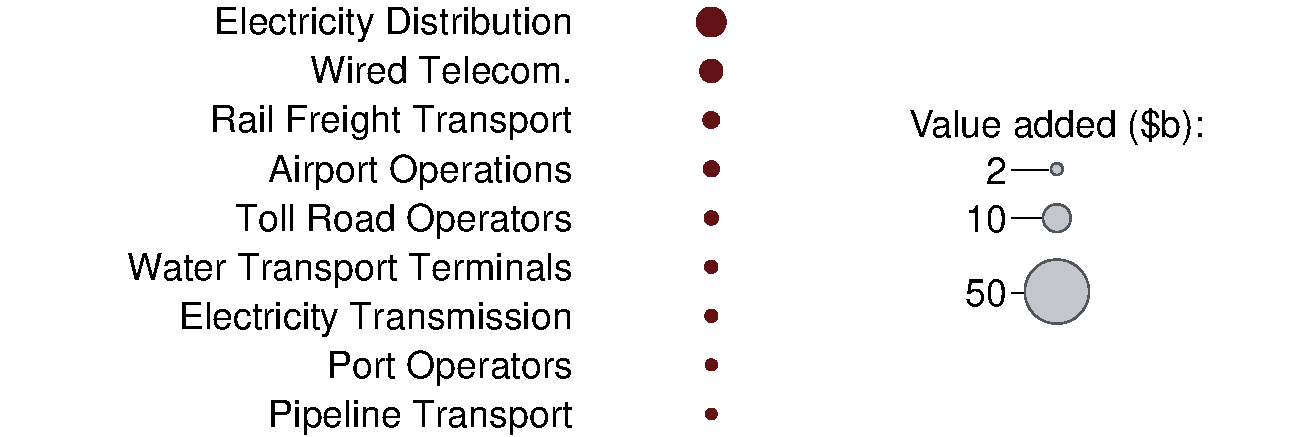
\includegraphics{atlas/NM_conc}

    \vspace{4pt}

    \units{Barriers to entry: scale-economy sectors}
    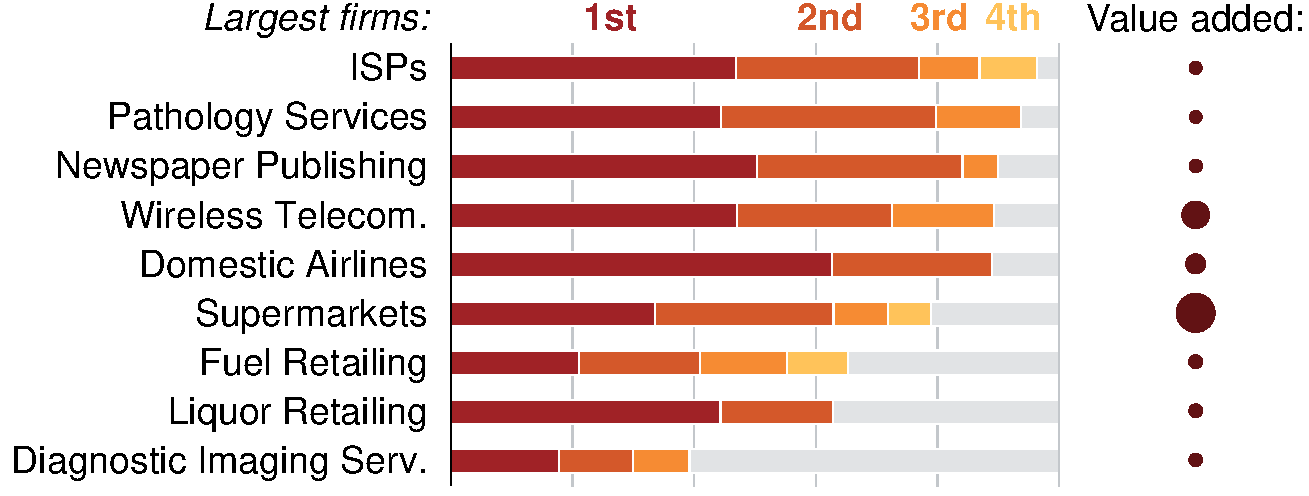
\includegraphics{atlas/SE_conc}

    \vspace{4pt}

    \units{Barriers to entry: heavily-regulated sectors}
    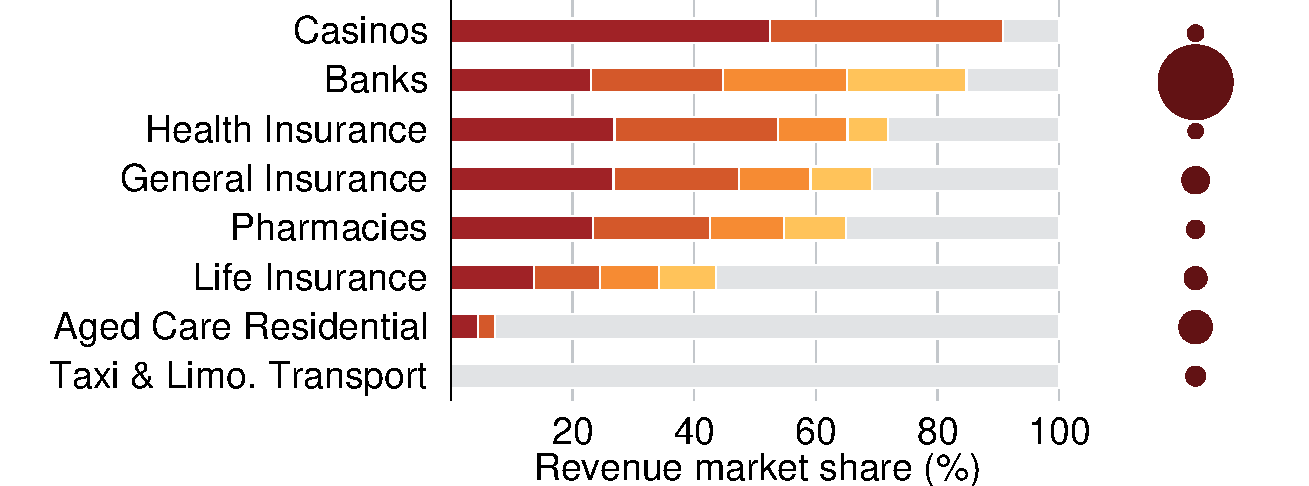
\includegraphics{atlas/HR_conc}
    \end{minipage}
    \hfill
    \begin{minipage}[t][\textheight]{\columnwidth}
        \vspace{-8pt}

    \units{Low barriers to entry}
    \includegraphics[page=2]{atlas/ChartsL}
    \end{minipage}
    \vspace{-56pt}
    \note{`Largest firms' excludes those with less than 5\% market share. \hspace{150pt} Source: Grattan analysis of \textcite{IBISWorldIndustry2017}.}
  \end{figure*}

\Vref{fig:concentration-by-barriers} shows the largest sectors by value added in each sector group, sorted by concentration. The largest \textbf{natural-monopoly} sectors are electricity distribution, wired telecom, rail freight transport, airports, and toll roads. Others include water transport terminals, electricity transmission, port operators, and pipeline transport.%

While the local market share of the largest firms in these sectors is typically 100 per cent, there are a few sectors in which very large local markets have more more than one player, such as container ports. While not shown in \Cref{fig:concentration-by-barriers}, natural-monopoly sectors are also highly concentrated at a national level.

The largest sectors with \textbf{economies of scale} include supermarkets, wireless telecoms, domestic airlines, fuel retailing, and liquor retailing. Many of these sectors are highly concentrated. Smaller sectors in this group include diagnostic imaging, newspaper publishing, internet service provision, pathology services,  passenger car rental, delivery services, ready-mixed concrete, internet publishing (which includes online platforms for job and house advertisements), and sports administrative services (which includes the Australian Football League).

% Supermarkets and mobile phone services (wireless telecommunications) are two of the largest sectors with network effects. Supermarkets benefit from networks of suppliers, warehouses, retail stores and marketing. Mobile operators need a network of towers to support their service, too many providers would have excess capacity and increase average costs. Duplicating these networks is costly and is a deterrent to new entrants. If the Australian economy reaches a size that can support more networks, new entrants may be enticed into these sectors.

% Regulation of these industries is often through merger restrictions and misuse of market power. This is intended to maintain competitive pressure in the interest of the consumer. But it has to be balanced against the potential efficiencies a larger firm might have, and the benefits this could provide consumers.

% Industries with network effects are the most interesting for international comparisons. Different regulatory environments could impact the level of industry concentration.

The largest \textbf{heavily-regulated} sector, by far, is banking, with about \$65 billion in value added. Other large regulated sectors are residential aged care, general insurance, life insurance, taxi \& limo transport, and pharmacies. Smaller sectors include casinos, health insurance, free-to-air TV, sports betting, and radio broadcasting. Many of these sectors are highly concentrated.

There are many large \textbf{low-barriers-to-entry} sectors. Few of them are concentrated (right chart, \Cref{fig:concentration-by-barriers}).

\newpage
\section{What this report does}

This report evaluates the evidence on competitive pressure in Australia. Is competitive pressure too low? Is it declining? Do firms in concentrated markets or in sectors protected by barriers to entry earn higher profits? How large might the economic costs be? 

Because the report looks right across the non-traded private economy, the level of detail is much lower than would be undertaken in a competition `market study', which might focus on a single sector, or split it out into smaller markets.%
\footnote{For example: \textcites{ACCCCommsMarketStudyDraft2017}{ACCCNewCarMarketStudyDraft2017}.}

\Chapref{chap:international} compares market concentration in some large, concentrated Australian sectors with concentration in those sectors in other economies.

%\newpage

\Chapref{chap:trends} assesses trends in concentration for some major sectors, as well as available data for others, and reviews other evidence on whether competitive pressure has weakened.

\Chapref{chap:profits} examines how profitability is affected by market concentration and barriers to entry.%
%\footnote{Profitability is a common yardstick that captures whether firms are able to price above their costs. It adjusts for the cost and depreciation of capital, and can be adjusted for risk, so it is well suited to comparing different sectors. An alternative measure, the margin of prices above marginal cost, also tend to be higher when firms have market power, but it is not useful when comparing markets for different products or services, because fixed costs (including depreciation) vary markedly from sector to sector.}

% \end{smallbox}

\Chapref{chap:welfare} then draws out possible implications for the overall economic costs of market power.

\Chapref{chap:policy} makes recommendations for policy directions that will help to increase competitive pressure. 
